\documentclass[a4,portrait]{seminar}
\usepackage{amsthm,amsmath,amssymb}
\usepackage{pifont}
\usepackage[spanish]{babel}
\usepackage{times}
\usepackage[dvips]{graphicx}
\usepackage{color}

\newtheorem{thm}{Teorema}
\begin{document}

\title{Generalizaciones del Teorema de Weierstrass}

\date{}
\maketitle

\raggedslides[0pt]

\thispagestyle{empty}

\begin{slide*}


\begin{thm}
    \textbf{Weierstrass cl\'asico.} Sea $f$ una funci\'on continua del intervalo $[a,b]$ en
    $\mathbb{R}$. Entonces $f$ alcanza un m\'aximo y un m\'inimo.
\end{thm}


\vspace{2cm}
\definecolor{amar}{gray}{.9}
\fcolorbox{amar}{amar}{

\begin{minipage}[c][3cm][c]{.9\linewidth}
 \textbf{Objetivo de la
clase:} Encontrar condiciones necesarias y suficientes sobre un
conjunto $K$ de un espacio m\'etrico $(X,d)$ de modo tal que toda
funci\'on continua alcance un m\'aximo y un m\'inimo sobre $K$.
\end{minipage}
}

\end{slide*}


\begin{slide*}

\begin{center}
\begin{large}
\textbf{?`Por qu\'e nos planteamos esto?}
\end{large}
\end{center}
\definecolor{amar}{gray}{.9}
{\raggedleft
\begin{minipage}[l]{7cm}
\begin{quote}
\emph{\small <<Nada ocupa un lugar en el mundo que no pueda ser
entendido como alg\'un m\'aximo o m\'inimo.>>}

{\raggedleft\small L. Euler\par}
\end{quote}
\end{minipage}\par
}






\begin{itemize}
    \item[\ding{226}]
        \emph{Principio de m\'inima acci\'on o Principio  de Hamilton.}
        Pensemos  un sistema
        mec\'anico caracterizado por las coordenadas $q=q_1,...,q_s$.
        Por ejemplo la posici\'on de $s/3$ puntos en el espacio.
        Este pricipio postula la existencia de una funci\'on
        \[
            L(t,q_1,...,q_s,\dot{q}_1,...,\dot{q}_s),
        \]
        que caracteriza al sistema en el siguiente sentido. Supongamos que en
        los instantes $t=t_1$ y $t=t_2$ tenemos
        determinadas las coordenadas  $q$, $q(t_1)=q^1$ y
        $q(t_2)=q^2$. Entonces, entre $t_1$ y $t_2$ el
        sistema evolucionar\'a de modo tal que la integral
        \[
            S=\int_{t_1}^{t_2}L(t,q_1,...,q_s,\dot{q}_1,...,\dot{q}_s)dt
        \]
        sea m\'inima.



\end{itemize}




\end{slide*}











\begin{slide*}

\begin{center}
\begin{large}
    \textbf{Conjuntos Compactos}
\end{large}
\end{center}
Recordemos algunas definiciones. Sea $(X,d)$ un espacio m\'etrico.
\definecolor{amar}{gray}{.9}
\begin{itemize}
    \item[\ding{226}] Un conjunto $K\subset X$ se llamar\'a
    \colorbox{amar}{compacto} si todo cubrimiento por abiertos relativos  de $K$ tiene un
    subcubrimiento finito. Es decir, si
    $K = \bigcup_{\lambda\in\Lambda}G_{\lambda}$, con
    $G_{\lambda}$ abierto en $K$ $\forall\lambda$, entonces existe un
    conjunto finito $\Lambda_0\subset\Lambda$ tal que
    $K=\bigcup_{\lambda\in\Lambda_0}G_{\lambda}$.

    \item[\ding{226}] Un conjunto $K\subset X$ se llama
    \colorbox{amar}{precompacto} si para cada $\epsilon>0$ podemos cubrir $K$ por
    un conjunto finito de bolas de radio $\epsilon$ y centro perteneciente a $K$.

    \item[\ding{226}] Un espacio m\'etrico se dice \colorbox{amar}{completo} si
    toda sucesi\'on de Cauchy es convergente.

\end{itemize}

\fcolorbox{amar}{amar}{
\begin{minipage}[c][1cm][c]{.95\linewidth}
\begin{thm}
    Un conjunto $K$ es compacto si, y solo si, es precompacto y
    completo.
\end{thm}
\end{minipage}
}
\end{slide*}



\begin{slide*}
\begin{center}
{\large \textbf{La precompacidad es condici\'on necesaria}}
\end{center}

\definecolor{amar}{gray}{.9}
\fcolorbox{amar}{amar}{
        \begin{minipage}[c][2cm][c]{.95\linewidth}
            \begin{thm}
                    Sea $(X,d)$ un espacio m\'etrico y $K\subset X$.
                    Supongamos que toda funci\'on continua, alcanza un m\'aximo (y por
                    ende un m\'inimo) sobre $K$, entonces $K$ es precompacto.
            \end{thm}
        \end{minipage}
}
\begin{proof}
\setlength{\parskip}{2\parskip}


Supongamos  $K$ no  precompacto.


Existe $\epsilon>0$ tal que $K$ no se puede cubrir por una
cantidad finita de bolas de radio $\epsilon$.

Elijamos $x_1\in K$.

Como $B(x_1,\epsilon)\nsupseteq K$, tomemos $x_2\in
K-B(x_1,\epsilon)$.


De la misma forma elegimos $x_3\in K-B(x_1,\epsilon)\cup
B(x_2,\epsilon)$.

Continuamos de esta forma, producimos una sucesi\'on $x_n$ tal que
\[
    x_n\in K-B(x_1,\epsilon)\cup\dots\cup B(x_{n-1},\epsilon).
\]

Consideremos $\delta=\epsilon/2$.

Tenemos que, para $i\neq j$, $B(x_i,\delta)\cap
B(x_j,\delta)\neq\emptyset$ (\textbf{Ejercicio})



\setlength{\unitlength}{40mm}
\begin{figure}[h]
    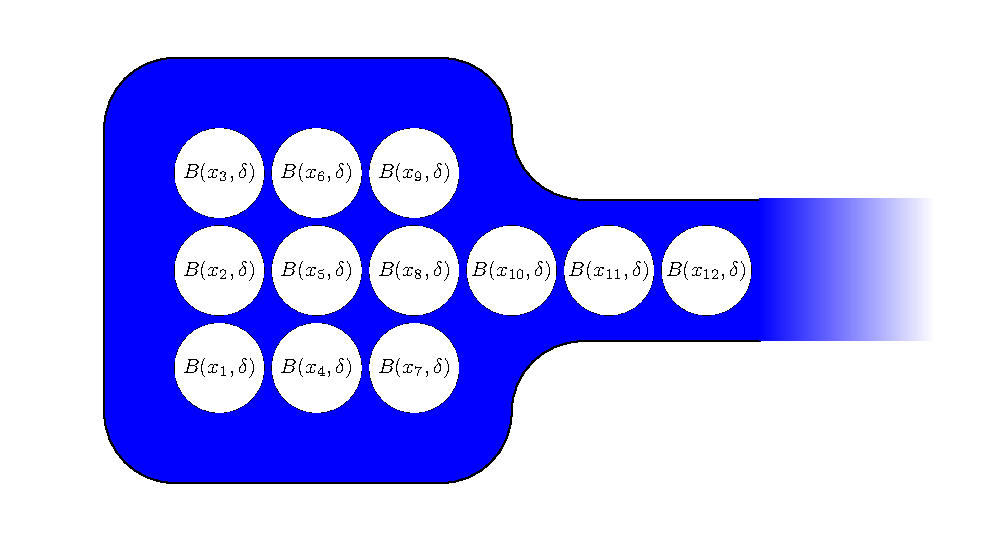
\includegraphics[height=1\unitlength,width=1.8314\unitlength]{figura2.eps}
\caption{Bolas $B(x_j,\delta)$}\label{bolitas}
\end{figure}


Ahora consideremos las funciones:
\[
    f_k(x)=\max\{\delta-d(x,x_k), 0\}
\]

\begin{enumerate}
    \item  $f_k$ es continua, pues es un m\'aximo de funciones
            continuas.
    \item  $f(x)=0$ si $x\notin B(x_k,\delta)$
    \item  $0\leq f _k\leq\delta$ y $f_k(x_k)=\delta$.
\end{enumerate}
 Definimos:

\[
    f(x):=\sum\limits_{k=1}^{\infty}\biggl(1-\frac{1}{k}\biggr) f_k(x).
\]


\setlength{\unitlength}{70mm}
\begin{figure}[h]
    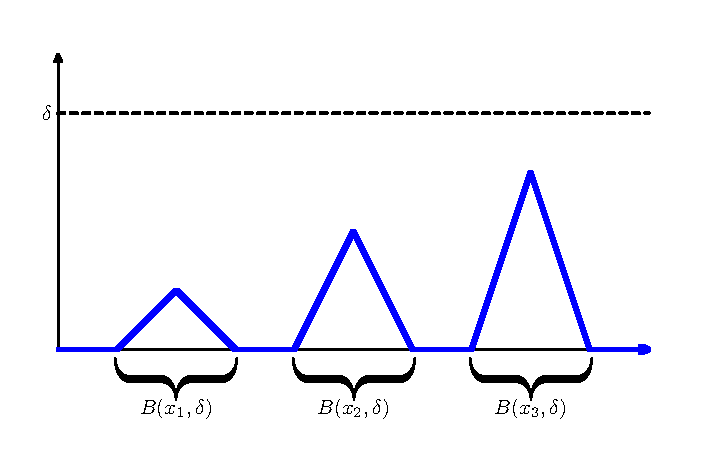
\includegraphics[width=.9\unitlength,height=0.57\unitlength]{figura3.eps}
\caption{Funci\'on $f$}\label{funcnoacot}
\end{figure}

$f$   no alcanza un m\'aximo, pues $0 \leq f<\delta$ y
$f(x_k)=\delta (1-\frac{1}{k})\to\delta$ cuando $k\to\infty$.

\newpage

\textbf{Afirmaci\'on} si $x^*\in K$ existe un $\eta=\eta(x^*)>0$
tal que para $d(x,x^*)<\eta$


\begin{equation}\label{ecua}
    |f(x)-f(x^*)|\leq d(x,x^*).
\end{equation}

Por lo tanto $f$ es continua.


Demostremos \eqref{ecua}.

Sea $x^*\in K$.

\begin{enumerate}

    \item Si $\exists k$ con $x^*\in\ B(x_k,\delta)$ \textbf{Ejercicio}

    \item Supongamos $x^*\notin B(x_k,\delta)$, $\forall k$.

            Sea $\delta >\eta>0$.

            Supongamos que $d(x,x^*)<\eta$.

    \begin{enumerate}

        \item Si $x\notin B(x_k,\delta)$, $\forall k$, entonces
                \[
                    f(x)=f(x^*)=0.
                \]
                Por ende \eqref{ecua} es cierta.



        \newpage

        \item Si $\exists k$ con $x\in B(x_k,\delta)$, entonces
        \[
            \delta \leq d(x_k,x^*)\leq
            d(x_k,x)+d(x,x^*).
        \]
        Entonces
        \begin{equation}
        \begin{split}
            |f(x)-f(x^*)|&=f(x)\\
            &=\biggl(1-\frac{1}{k}\biggr)\bigl(\delta-d(x,x_k)\bigr)\\
            &<d(x^*, x).
        \end{split}\notag
        \end{equation}
    \end{enumerate}
\end{enumerate}
\end{proof}













\end{slide*}

\begin{slide*}

\begin{center}
{\large \textbf{La completitud es necesaria}}
\end{center}


\definecolor{amar}{gray}{.9}
\fcolorbox{amar}{amar}{
        \begin{minipage}[c][2cm][c]{.95\linewidth}
            \begin{thm}
                    Sea $(X,d)$ un espacio m\'etrico y $K\subset X$.
                    Supongamos que toda funci\'on continua, alcanza un m\'aximo (y por
                    ende un m\'inimo) sobre $K$, entonces $K$ es completo.
            \end{thm}
        \end{minipage}
}

\begin{proof}  Supongamos $K$ no completo.

Sea $\{x_n\}$ una sucesi\'on de Cauchy en $K$ que no converge.

Definamos
\[
    f(x):=\lim\limits_{n\to\infty}d(x,x_n).
\]

\textbf{Afirmaci\'on:} El l\'imite anterior existe.

Se prueba as\'i. La desigualdad
\[
    |d(x,x_n)-d(x,x_m)|\leq d(x_n,x_m),
\]
implica  que la sucesi\'on $d(x,x_n)$ es de Cauchy en
$\mathbb{R}$.

Como $\mathbb{R}$ es completo, la sucesi\'on $d(x,x_n)$ es
convergente.

Veamos que $f$ es continua y de hecho Lipschitz.

\begin{equation}
\begin{split}
|f(x)-f(y)| &
=|\lim\limits_{n\to\infty}d(x,x_n)-\lim\limits_{n\to\infty}d(y,x_n)|\\
&= \lim\limits_{n\to\infty}|d(x,x_n)-d(y,x_n)|\\
&\leq d(x,y).
\end{split}\notag
\end{equation}

Veamos que $f$ no alcanza un m\'inimo.

Si $\epsilon>0$ existe $N\in\mathbb{N}$ tal que
\[
    d(x_n,x_m)<\epsilon\quad\text{para}\,\,n,m>N.
\]

Haciendo $m\to\infty$ obtenemos

\[
    f(x_n)=\lim\limits_{m\to\infty}d(x_n,x_m)\leq\epsilon.
\]

Esto implica que

\[
    \inf\limits_{x\in K}f(x)=0.
\]

Pero, para $x\in K$ tenemos que $f(x)\neq 0$, de lo contrario
$\{a_n\}$ converger\'ia. As\'i $f$ no tiene m\'inimo.


\end{proof}






\end{slide*}




\begin{slide*}

\begin{center}
{\large \textbf{Compacto es necesario y suficiente}}
\end{center}

\definecolor{amar}{gray}{.9}

\fcolorbox{amar}{amar}{
        \begin{minipage}[c][1.3cm][c]{0.95\linewidth}
                \begin{thm} Sea $K$ un subconjunto compacto de $X$.
                Toda funci\'on continua alcanza un m\'aximo (o un m\'inimo) sobre $K$
                si, y s\'olo si,  $K$ es compacto.
                \end{thm}
        \end{minipage}
        }

\begin{proof} S\'olo falta la suficiencia.

Supongamos $K$ compacto.



S\'olo probaremos   que $f$ alcanza un m\'aximo, aplicando este
resultado a $-f$ demostramos que $f$ alcanza un m\'inimo.


Supongamos que $f$ no alcanza un m\'aximo.

Para cada $y\in f(K)$ definimos el conjunto

\[
    G_y:=f^{-1}\bigl((-\infty,y)\bigr)=\{x\in K:f(x)<y\}.
\]

\begin{center}
\begin{figure}[h]
\setlength{\unitlength}{46mm}
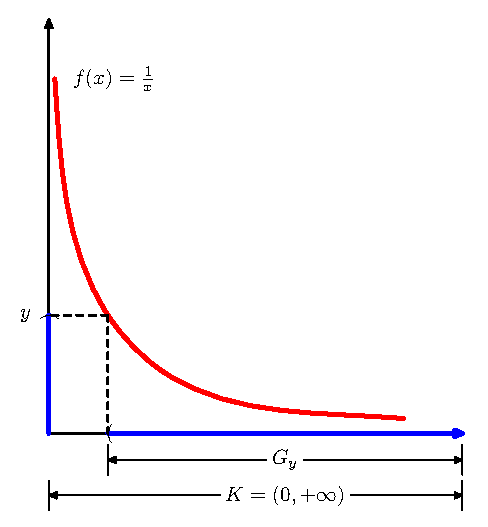
\includegraphics[height=1\unitlength,width=0.98\unitlength]{figura1.eps}
\caption{Conjuntos $G_y$}\label{figura1}
\end{figure}
\end{center}

\begin{itemize}
    \item[\ding{226}]
        Los conjuntos $G_y$ son abiertos relativos a $K$, pues $f$ es continua.
    \item[\ding{226}]
         $\{G_y\}_{y\in f(K)}$ es un cubrimiento de
        $K$.

        Sea $x\in K$.

         $x$ no es un punto de m\'aximo $\Rightarrow$
         $\exists z\in K$ tal que

         \[
          f(x)<f(z)
         \]

         Esto implica que $x\in G_{f(z)}$.

    \item[\ding{226}]
        Si $y_1<y_2\Rightarrow G_{y_1}\subset G_{y_2}$
\end{itemize}

 $K$ es compacto $\Rightarrow$ existe un subconjunto finito\\
$\{y_1,...,y_n\}\subset f(K)$ tal que
\begin{equation}\label{cubre}
    K=G_{y_1}\cup\dots\cup G_{y_n}.
\end{equation}
Sea $y^*=\max\{y_1,...,y_n\}$.

 Se tiene que $y^*\in f(K)$.

 Por la igualdad \eqref{cubre},
 \[
    \forall x\in K: f(x)<y^*.
 \]

Lo que es una contradicci\'on.
\end{proof}


\end{slide*}






\end{document}
